\section{Electrokinetics}

\subsection{Basic concepts}

\begin{frame}{Sample system - a 2D channel}
Example of a ``simple'' electrokinetic system:

\begin{figure}
\begin{center}
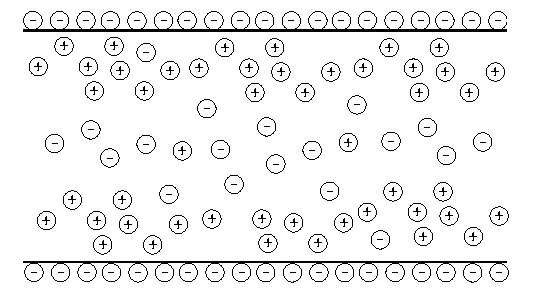
\includegraphics[width=0.7\textwidth]{../fig/channel.pdf}
\end{center}
\end{figure}

The solution contains charges, the walls are charged, external
electric/force fields may be present...

\end{frame}

\begin{frame}{Electrical double layers (EDLs)}
Ionic solution in contact with a charged object $\implies$ EDL

\begin{figure}
\begin{center}
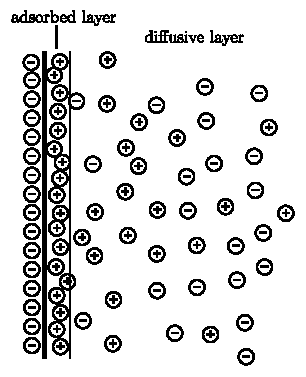
\includegraphics[width=0.5\textwidth]{../fig/edl.pdf}
\end{center}
\end{figure}

\end{frame}

\subsection{Modelling approach}

\begin{frame}{Involved equations}

\begin{itemize*}

\item The electric potential from the charge presence. Poisson's
  equation for electrostatics:
\begin{equation}\label{eq:pb}
\nabla^2\psirm = -\frac{\rho_e}{\epsilon_r \epsilon_0}
\end{equation}


\item The transport of charges due to diffusion, advection and the
  presence of electric fields. The Nernst-Planck equation:
\begin{equation}\label{eq:et:np}
\dfrac{\partial \C}{\partial t} = \nabla \cdot \left [
 D\nabla \C - \C\ubf + \frac{zq_eD}{k_BT}\C\nabla\psirm
\right]
\end{equation}

\item The flow field, affected by electrokinetic
  effects. (Incompressible) Navier-Stokes equations:
\begin{equation}\label{eq:et:ns_incompressible}
 \nabla \cdot \ubf = 0
\end{equation}
and

\begin{equation}\label{eq:et:ns_mom}
\rhorm \left (\dfrac{\partial \ubf}{\partial t} +
  \ubf \cdot \nabla \ubf 
  \right ) = - \nabla \Prm  + \mu \nabla^2 \ubf + \F
\end{equation}


\end{itemize*}

\end{frame}

\begin{frame}
\begin{figure}
\begin{center}
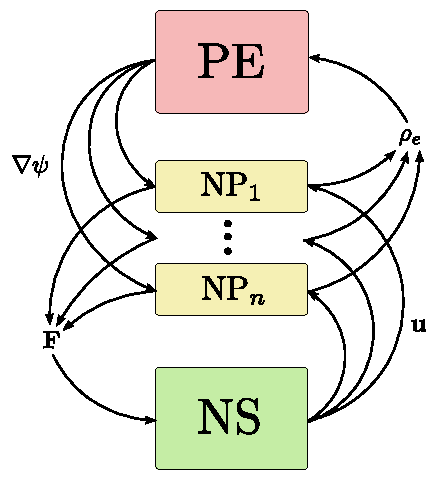
\includegraphics[width=0.5\textwidth]{../fig/coupling.pdf}
\end{center}
\caption{Visualisation of the coupling between the three equations
  present in the model. Poisson's equation (PE), The set of
  Nernst-Planck equations (NP$_1$ ... NP$_n$) for the different ion
  species and the Navier-Stokes equations (NS). The dependencies have
  also be marked with arrows indicating what quantities for a certain
  equation that are needed from an other.}
\label{fig:coupling}
\end{figure}
\end{frame}

\subsection{Some electrokinetic phenomena}

\begin{frame}{The electroviscous effect}

\begin{equation}
\J = -  \sigma_c \nabla \phi  
\end{equation}

\begin{equation}
\F = - \rho_e \nabla \phi
\end{equation}

\begin{figure}
\begin{center}
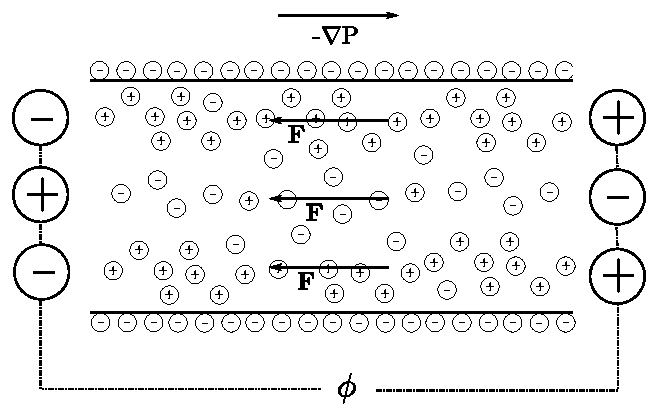
\includegraphics[width=0.7\textwidth]{../fig/channel_electroviscous.pdf}\\
Streaming potential
\end{center}
\end{figure}

\end{frame}

\begin{frame}{Electroosmosis}

\begin{equation}
\F = \rhorm_e \E
\end{equation}

\begin{figure}
\begin{center}
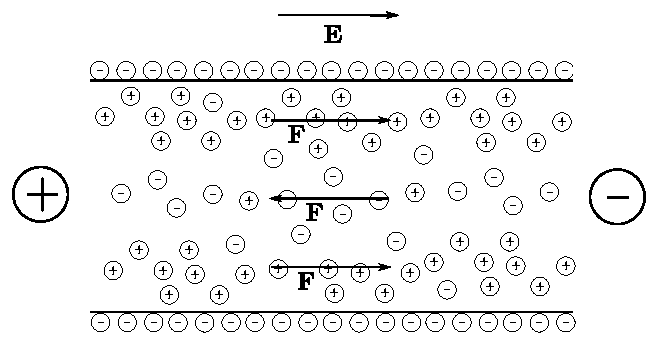
\includegraphics[width=0.7\textwidth]{../fig/channel_electroosmosis.pdf}
\end{center}
\end{figure}

\end{frame}

\begin{frame}{Boundary conditions}
Boundary conditions at (charged) walls, $\Gamma$

\begin{itemize*}
\item Poisson's equation: fixed surface charge, $\sigma_s$
\begin{equation}\label{eq:et:fix_c}
\nabla\psirm(\x) \cdot \n =
-\frac{\sigma_s(\x)}{\epsilon_0\epsilon_r}\;,\;\; \x \in \Gamma
\end{equation}

\item Nernst-Planck: zero flux through wall
\begin{equation}\label{eq:et:j0}
\J(\x) \cdot \mathbf{n} = 0 \;,\;\; \x \in \Gamma
\end{equation}

\item Navier-Stokes: no-slip
\begin{equation}
\ubf(\x) = 0 \;,\;\; \x \in \Gamma
\end{equation} 

\end{itemize*}
\end{frame}
